\documentclass[10pt]{beamer}

% ------------------------------------------------------------------------
% Carga de tu preámbulo personalizado (preamble.tex).
% Asegúrate de tenerlo en la misma carpeta para que \input funcione.
% ------------------------------------------------------------------------
\usetheme[progressbar=frametitle]{metropolis}
\usepackage{appendixnumberbeamer}
\usepackage{fancyvrb}
\usepackage{booktabs}
\usepackage[scale=2]{ccicons}
\usepackage{pgfplots}
\usepgfplotslibrary{dateplot}
\usepackage{type1cm}
\usepackage{lettrine}
\usepackage{ragged2e}
\usepackage{xspace}
\newcommand{\themename}{\textbf{\textsc{metropolis}}\xspace}
\usepackage{graphicx} % Allows including images
\usepackage{booktabs} % Allows the use of \toprule, \midrule and \bottomrule in tables
\usepackage[utf8]{inputenc} %solucion del problema de los acentos.
\usepackage{xcolor}
\definecolor{LightGray}{gray}{0.9}

\usepackage{minted}
\usemintedstyle{tango}
\newcommand{\mypyfile}[1]{\inputminted[linenos=true, fontsize=\footnotesize, frame=lines, framesep=5\fboxrule,framerule=1pt]{python}{#1}}

\setminted[python]{breaklines,frame=lines,framesep=2mm,baselinestretch=1.2,bgcolor=LightGray,linenos, fontsize=\footnotesize} % obeytabs=true, tabsize=2, showtabs=true}

%%%%%%%%%%%%%%%%%%%%%%%%%%%%%%%%%%%%%%%%%%%%%%%%%%%%%%%%%%%%%%%%%%%%%%%%%%%%%%%%%%%%%%
\setbeamercolor{progress bar}{fg=blue!50!black,bg=white!50!black}
\setbeamercolor{title separator}{fg=red!50!black,bg=white!50!black}
\setbeamercolor{frametitle}{fg=white!80!black,bg=red!50!black}
\title[PCFI161]{Programaci\'on para F\'isica y Astronom\'ia}
\subtitle{Departamento de Física.}

\newcommand{\myfront}{
\author[PCFI161]{Corodinadora: C Loyola \\ Profesoras/es C Loyola / C Femenías / Y Navarrete / C Ruiz}
\institute[UNAB]{Universidad Andrés Bello}
\date{Primer Semestre 2025}
}

\titlegraphic{%
  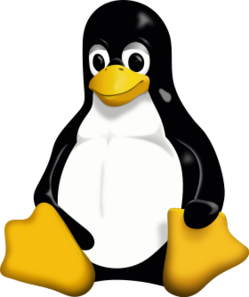
\includegraphics[width=.08\textwidth]{logo-tux.png}\hfill
  
\includegraphics[width=.3\textwidth]{logo-unab.png}\hfill
  
\includegraphics[width=.08\textwidth]{logo-python.png}
}

\makeatletter
\setbeamertemplate{title page}{
  \begin{minipage}[b][\paperheight]{\textwidth}
    \vfill%
    \ifx\inserttitle\@empty\else\usebeamertemplate*{title}\fi
    \ifx\insertsubtitle\@empty\else\usebeamertemplate*{subtitle}\fi
    \usebeamertemplate*{title separator}
    \ifx\beamer@shortauthor\@empty\else\usebeamertemplate*{author}\fi
    \ifx\insertdate\@empty\else\usebeamertemplate*{date}\fi
    \ifx\insertinstitute\@empty\else\usebeamertemplate*{institute}\fi
    \vfill
    \ifx\inserttitlegraphic\@empty\else\inserttitlegraphic\fi
    \vspace*{1cm}
  \end{minipage}
}
\makeatother


\makeatletter
\setlength{\metropolis@titleseparator@linewidth}{2pt}
\setlength{\metropolis@progressonsectionpage@linewidth}{2pt}
\setlength{\metropolis@progressinheadfoot@linewidth}{2pt}
\makeatother


\begin{document}

% ------------------------------------------------------------------------
% Portada de la Presentación
% ------------------------------------------------------------------------
\myfront{}

% ------------------------------------------------------------------------
% Slide 1: Título de la Sesión
% ------------------------------------------------------------------------
\begin{frame}
  \titlepage
  % Ejemplo:
  % \title{Semana 13 - Sesión 2 (Sesión 26): Problema Evaluado (25-30 min) ligado a Temas de la Semana 12}
\end{frame}

% ------------------------------------------------------------------------
% Slide 2: Índice / Tabla de Contenidos
% ------------------------------------------------------------------------
\begin{frame}
  \frametitle{Resumen - Semana 13, Sesión 2 (Sesión 26)}
  \tableofcontents
\end{frame}

% ------------------------------------------------------------------------
% Configuración de bloques
% ------------------------------------------------------------------------
\metroset{block=fill}

% ----------------------------------------------------------------------------------------
% SECCIÓN 1: Introducción y Conexión con la Semana 12
% ----------------------------------------------------------------------------------------
\section{Introducción y Contexto}

% ------------------------------------------------------------------------
% Slide 3: Repaso de la Semana 12
% ------------------------------------------------------------------------
\begin{frame}{Contexto de la Semana 12}
  \begin{itemize}
    \item \textbf{Semana 12, Sesión 1 (Sesión 23)}:
      \begin{itemize}
        \item Lanzamiento formal de proyectos integradores (requisitos, equipos).
        \item Introducción a \textbf{SciPy} (o Sympy) como herramienta para ecuaciones diferenciales, optimización, etc.
      \end{itemize}
    \item \textbf{Semana 12, Sesión 2 (Sesión 24)}:
      \begin{itemize}
        \item \textbf{Problema a Evaluar} sobre POO (composición) y Matplotlib (bar plot), conectando con la Semana 11.
        \item Práctica de subir a CANVAS en 25-30 minutos.
      \end{itemize}
    \item \textbf{Objetivo de hoy (Semana 13, Sesión 2)}:
      \begin{itemize}
        \item Resolver un \textbf{nuevo Problema Evaluado} (25-30 min) relacionado a \textbf{Semana 12}, es decir, la introducción a SciPy/Sympy o el arranque de proyectos.
        \item Subir la solución a CANVAS y discutir brevemente.
      \end{itemize}
  \end{itemize}
\end{frame}

% ------------------------------------------------------------------------
% Slide 4: Objetivos de la Sesión 26
% ------------------------------------------------------------------------
\begin{frame}{Objetivos de la Sesión 26}
  \begin{itemize}
    \item \textbf{Aplicar} conceptos o herramientas introducidas en Semana 12 (por ejemplo, \textbf{SciPy} integraciones, ODEs, optimizaciones) o elementos del proyecto (POO + SciPy).
    \item \textbf{Evaluar} el desempeño en un problema corto (25-30 min), subido a \textbf{CANVAS} en grupo.
    \item \textbf{Retroalimentar} fallas o dificultades al usar SciPy/Sympy o la integración con NumPy/Matplotlib.
    \item \textbf{Avanzar} en la consolidación de las herramientas para el proyecto final.
  \end{itemize}
\end{frame}

% ----------------------------------------------------------------------------------------
% SECCIÓN 2: Problema a Evaluar (25-30 min)
% ----------------------------------------------------------------------------------------
\section{Problema a Evaluar}

% ------------------------------------------------------------------------
% Slide 5: Descripción del Problema
% ------------------------------------------------------------------------
\begin{frame}{Problema a Evaluar: Uso de SciPy (o Sympy) y POO Básica}
  \textbf{Contexto (Semana 12):}  
  \begin{itemize}
    \item Vimos \textbf{SciPy} para integración, optimización, ODEs o \textbf{Sympy} para resolver expresiones simbólicas, derivadas.
    \item Se mencionó la posible \textbf{combinación} con POO.
  \end{itemize}

  \textbf{Tareas}:
  \begin{enumerate}
    \item Definir una \textbf{función} (o método de clase) que represente una \textbf{EDO} simple, por ejemplo \(\frac{dy}{dt} = -a \cdot y\) (decaimiento exponencial).
    \item Usar \textbf{SciPy} (\texttt{odeint} o \texttt{solve\_ivp}) para resolverla en un rango de \(\texttt{t}\).
    \item Graficar el resultado con \(\textbf{Matplotlib}\) (\texttt{plt.plot(t, solution)}) indicando la forma exponencial.
    \item (Opcional) Incluir una clase \texttt{DecayModel} con atributo \texttt{a} y método \texttt{solve(t0, y0, t\_range)}, integrando la idea de POO.
  \end{enumerate}
\end{frame}

% ------------------------------------------------------------------------
% Slide 6: Instrucciones y Formato de Entrega
% ------------------------------------------------------------------------
\begin{frame}{Instrucciones para la Evaluación}
  \begin{itemize}
    \item \textbf{Grupos} de 2-3 estudiantes (mismos equipos o asignados).
    \item Crear un \textbf{notebook} (Colab) o \textbf{script local} llamado \texttt{Eval\_Semana13\_Apellidos.ipynb}.
    \item \textbf{Desarrollo}:
      \begin{enumerate}
        \item Importar \(\texttt{scipy.integrate}\) (ej. \texttt{odeint}).
        \item Definir la EDO \(\texttt{dy/dt = -a*y}\) en una función Python.
        \item Resolver para un \(\texttt{a}\) dado, \(\texttt{y0}\) inicial, y rango de \(\texttt{t}\).
        \item Graficar la \textbf{solución} con \(\texttt{matplotlib}\).
        \item (Opcional) \textbf{Clase DecayModel} que encapsule \(\texttt{a}\) y la función EDO, con un método \texttt{solve}.
      \end{enumerate}
    \item \textbf{Subir} el archivo a \textbf{CANVAS} en \textbf{25-30 min}.
  \end{itemize}
\end{frame}

% ------------------------------------------------------------------------
% Slide 7: Pautas de Evaluación
% ------------------------------------------------------------------------
\begin{frame}{Pautas de Evaluación}
  \textbf{Criterios}:
  \begin{itemize}
    \item \textbf{Funcionalidad} (40\%): la EDO se resuelve sin errores y se grafica el resultado.
    \item \textbf{Uso apropiado de SciPy} (20\%): \(\texttt{odeint}\) o \(\texttt{solve\_ivp}\) con parámetros correctos, \(\texttt{(t, y)}\) coherentes.
    \item \textbf{Visualización} (20\%): \(\texttt{plt.plot}\) con eje X de \textbf{tiempo} y eje Y de \textbf{solución}, con título y ejes rotulados.
    \item \textbf{Organización / Clase opcional} (20\%): si implementan \textbf{DecayModel}, \_\_init\_\_, \texttt{solve}, etc. O al menos un código ordenado, con comentarios.
  \end{itemize}
\end{frame}

% ------------------------------------------------------------------------
% Slide 8: Tiempo de Desarrollo (25-30 min)
% ------------------------------------------------------------------------
\begin{frame}{Tiempo de Desarrollo}
  \begin{block}{}
    \huge{\textbf{Tienen 25-30 minutos para resolver y subir a CANVAS.}}
  \end{block}
  \vspace{0.3cm}
  \textbf{Sugerencias}:
  \begin{itemize}
    \item Revisar ejemplo de \textbf{odeint} con \texttt{def model(y, t, a): return -a*y}.
    \item Asegurarse de \textbf{importar} \(\texttt{matplotlib.pyplot as plt}\) y \(\texttt{from scipy.integrate import odeint}\).
    \item Probar distintos valores de \textbf{a} y \textbf{y0} para ver la curva.
    \item (Opcional) Crear la clase \texttt{DecayModel(a)}, con \texttt{def solve(self, y0, t\_span): ...}.
  \end{itemize}
\end{frame}

% ----------------------------------------------------------------------------------------
% SECCIÓN 3: Trabajo y Discusión
% ----------------------------------------------------------------------------------------
\section{Trabajo y Discusión}

% ------------------------------------------------------------------------
% Slide 9: Espacio de Resolución y Entrega
% ------------------------------------------------------------------------
\begin{frame}{Espacio de Resolución}
  \begin{itemize}
    \item \textbf{Trabajen en voz baja}, cada grupo crea su notebook o script.
    \item Preguntas puntuales a mí si hay bloqueo total.
    \item Subir a CANVAS antes de que finalice el tiempo (25-30 min).
  \end{itemize}
\end{frame}

% ------------------------------------------------------------------------
% Slide 10: Cierre de la Evaluación
% ------------------------------------------------------------------------
\begin{frame}{Entrega Final}
  \begin{block}{Subir a CANVAS}
    \begin{itemize}
      \item Un integrante sube el \textbf{notebook .ipynb} o \textbf{.py} dentro del tiempo establecido.
      \item Revisen que el \textbf{gráfico} y la \textbf{solución} estén mostrados correctamente.
      \item Comenten brevemente el código, param. de \texttt{a}, \texttt{y0}, etc.
    \end{itemize}
  \end{block}
  \vspace{0.3cm}
  \textbf{Al final}, haremos una breve \textbf{discusión} sobre resultados y dificultades.
\end{frame}

% ------------------------------------------------------------------------
% Slide 11: Discusión de Resultados
% ------------------------------------------------------------------------
\begin{frame}{Discusión Posterior}
  \begin{itemize}
    \item ¿Alguien tuvo problemas con \(\texttt{odeint}\) o \(\texttt{solve\_ivp}\)?
    \item ¿Cómo rotularon o personalizaron la gráfica?
    \item ¿Implementaron la \textbf{clase opcional}? ¿Cómo lo hicieron?
    \item ¿Dudas sobre integraciones más complejas?
  \end{itemize}
\end{frame}

% ------------------------------------------------------------------------
% Slide 12: Resumen de la Evaluación
% ------------------------------------------------------------------------
\begin{frame}{Resumen de la Evaluación}
  \begin{itemize}
    \item Actividad integró \textbf{SciPy} (odeint / solve\_ivp) de la Semana 12 y la idea de POO.
    \item Refuerza la metodología de \textbf{mini-evaluaciones} con entrega en CANVAS.
    \item Retroalimentación detallada se compartirá tras la corrección.
  \end{itemize}
\end{frame}

% ----------------------------------------------------------------------------------------
% SECCIÓN 4: Cierre de la Sesión y Próximos Pasos
% ----------------------------------------------------------------------------------------
\section{Conclusiones y Próximos Pasos}

% ------------------------------------------------------------------------
% Slide 13: Conclusiones de la Sesión 26
% ------------------------------------------------------------------------
\begin{frame}{Conclusiones de la Sesión 26}
  \begin{itemize}
    \item Realizamos un \textbf{Problema a Evaluar} usando \textbf{SciPy} (tema Semana 12).
    \item Vimos la importancia de la \textbf{visualización} de la solución numérica.
    \item Quien implementó POO (clase \texttt{DecayModel}) reforzó el diseño modular.
    \item Esto se vincula a proyectos que incluyan \textbf{cálculos diferenciales}, simulaciones, etc.
  \end{itemize}
\end{frame}

% ------------------------------------------------------------------------
% Slide 14: Próxima Sesión (Semana 14)
% ------------------------------------------------------------------------
\begin{frame}{Próximos Temas}
  \begin{itemize}
    \item \textbf{Semana 14}: Continuar revisando avances de proyectos, entregar avance 2 (si ese es el cronograma).
    \item Analizar dudas más profundas de \textbf{ODEs} en SciPy, \textbf{Sympy} simbólico, etc.
    \item Podríamos explorar \textbf{optimización} (\texttt{scipy.optimize}), \textbf{fft} (\texttt{scipy.fft}), etc.
  \end{itemize}
\end{frame}

% ------------------------------------------------------------------------
% Slide 15: Recursos Adicionales
% ------------------------------------------------------------------------
\begin{frame}{Recursos Adicionales}
  \begin{itemize}
    \item \href{https://docs.scipy.org/doc/scipy/reference/integrate.html}{\textbf{scipy.integrate}} - doc oficial.
    \item \href{https://matplotlib.org/3.3.0/tutorials/introductory/lifecycle.html}{\textbf{Matplotlib}} - explicación de la parte de figuras, ejes.
    \item \href{https://docs.python.org/3/tutorial/classes.html}{\textbf{POO}} - Repaso de \_\_init\_\_, etc.
    \item \textbf{CANVAS y Foros} - compartir repos y pedir apoyo.
  \end{itemize}
\end{frame}

% ------------------------------------------------------------------------
% Slide 16: Cierre de la Sesión
% ------------------------------------------------------------------------
\begin{frame}
  \Huge{\centerline{¡Excelente trabajo y hasta la próxima sesión!}}
  \vspace{0.5cm}
  \normalsize
  \begin{itemize}
    \item Revisen \textbf{Canvas} para feedback e información de sus proyectos.
    \item ¡Nos vemos en la Semana 14 con más desarrollo!
  \end{itemize}
\end{frame}

\end{document}

